\section*{CHAPTER 3. SYSTEM MODEL AND SIMULATION SETUP}
\addcontentsline{toc}{section}{\numberline{}CHAPTER 3. SYSTEM MODEL AND SIMULATION SETUP}

\setcounter{section}{3}
\setcounter{subsection}{0}
\setcounter{figure}{0}
\setcounter{table}{0}
\setcounter{equation}{0}

%============================================================%
\subsection{Introduction}

This chapter presents the system model and simulation methodology used to
evaluate the performance of OFDM and SC-FDMA transmission systems. Both
systems were implemented in MATLAB under identical transmission
conditions to ensure a fair comparison.

The simulations focus on two important performance metrics:

\begin{itemize}
    \item Bit Error Rate (BER)
    \item Peak-to-Average Power Ratio (PAPR)
\end{itemize}

A multipath Rayleigh fading channel with additive white Gaussian noise
(AWGN) was considered in the simulation. Zero Forcing (ZF) equalization
was applied at the receiver to compensate for channel distortion.

%============================================================%
\subsection{Overall System Model}

Both OFDM and SC-FDMA systems share highly similar transmission
architectures. The major difference is the introduction of a DFT spreading
operation in SC-FDMA before subcarrier mapping.

In OFDM, modulated symbols are directly mapped onto orthogonal
subcarriers and transformed into the time domain using the Inverse Fast
Fourier Transform (IFFT). In contrast, SC-FDMA first applies a DFT to the
modulated symbols, which spreads the information symbols across the
allocated subcarriers before OFDM modulation.

The OFDM transmitter structure can be summarized as:

\begin{center}
Bits $\rightarrow$ 16-QAM $\rightarrow$
Subcarrier Mapping $\rightarrow$
IFFT $\rightarrow$
Cyclic Prefix $\rightarrow$
Channel
\end{center}

Meanwhile, the SC-FDMA transmitter introduces an additional DFT
precoding stage:

\begin{center}
Bits $\rightarrow$ 16-QAM $\rightarrow$
DFT $\rightarrow$
Subcarrier Mapping $\rightarrow$
IFFT $\rightarrow$
Cyclic Prefix $\rightarrow$
Channel
\end{center}

At the receiver side, both systems perform cyclic prefix removal and FFT
processing to recover the transmitted subcarriers. Frequency-domain
equalization is then applied to compensate for multipath fading effects.

For SC-FDMA, an additional inverse DFT (IDFT) operation is required after
subcarrier demapping to recover the original symbol sequence.

\vspace{0.3cm}

\begin{figure}[H]
    \centering
    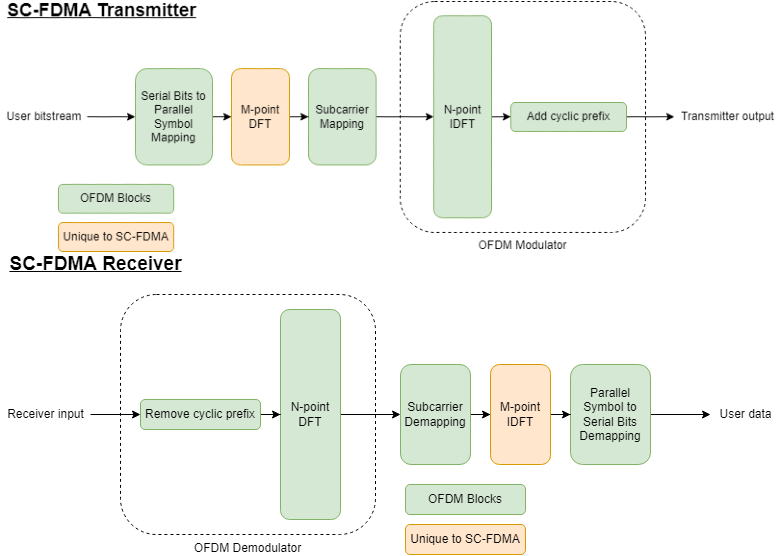
\includegraphics[width=0.95\textwidth]{Figures/system_model.png}
    \caption{\bfseries SC-FDMA transceiver structure based on OFDM modulation}
    \label{fig:system_model}
\end{figure}

In Figure \ref{fig:system_model}, the green processing blocks correspond
to conventional OFDM operations, while the orange blocks represent the
additional DFT spreading and despreading operations unique to SC-FDMA.

The additional DFT precoding stage gives SC-FDMA its
single-carrier-like characteristics and significantly reduces the
Peak-to-Average Power Ratio (PAPR) compared to conventional OFDM systems.

%============================================================%
\subsection{Simulation Parameters}

The simulation parameters used for both OFDM and SC-FDMA systems are
listed in Table \ref{tab:sim_parameters}.

\begin{table}[H]
\centering
\caption{Simulation Parameters}
\label{tab:sim_parameters}
\begin{tabularx}{0.9\textwidth}
{|>{\raggedright\arraybackslash}X|
 >{\centering\arraybackslash}X|}
\hline
\textbf{Parameter} & \textbf{Value} \\ \hline

FFT size ($N_{FFT}$) & 64 \\ \hline

Number of active subcarriers & 16 \\ \hline

Modulation scheme & 16-QAM \\ \hline

Cyclic Prefix length & 16 \\ \hline

Channel type & Multipath Rayleigh fading \\ \hline

Equalization method & Zero Forcing (ZF) \\ \hline

SNR range & 0 dB -- 20 dB \\ \hline

Number of transmitted blocks & 200000 \\ \hline

Channel taps & 3 \\ \hline

\end{tabularx}
\end{table}

A large number of transmitted blocks was selected to improve BER and CCDF
statistical accuracy.

%============================================================%
\subsection{Transmitted Signal Generation}

Random binary data were generated and grouped into symbols using 16-QAM
modulation.

The number of transmitted bits is calculated as:

\begin{equation}
N_b = N_{blk}\times N_{used}\times \log_2(M)
\end{equation}

where:
\begin{itemize}
    \item $N_{blk}$ is the number of transmitted blocks,
    \item $N_{used}$ is the number of active subcarriers,
    \item $M$ is the modulation order.
\end{itemize}

For OFDM, the modulated symbols were directly mapped onto active
subcarriers before IFFT processing.

For SC-FDMA, the symbols first passed through a DFT spreading stage:

\begin{equation}
X[m]=\sum_{n=0}^{M-1}
d[n]e^{-j\frac{2\pi mn}{M}}
\end{equation}

The resulting spread symbols were then mapped onto OFDM subcarriers and
transformed into the time domain using the IFFT.

%============================================================%
\subsection{Cyclic Prefix Insertion}

To mitigate inter-symbol interference caused by multipath propagation,
a cyclic prefix was inserted before transmission.

The cyclic prefix consists of copying the last portion of the OFDM symbol
and appending it to the beginning:

\begin{equation}
x_{CP}[n]=
[x(N-N_{CP}),\dots,x(N-1),x(0),\dots,x(N-1)]
\end{equation}

where:
\begin{itemize}
    \item $N$ is the FFT size,
    \item $N_{CP}$ is the cyclic prefix length.
\end{itemize}

The CP length was selected to exceed the channel delay spread in order to
preserve subcarrier orthogonality.

\vspace{0.3cm}

\begin{figure}[H]
    \centering
    \hspace*{-0.18\textwidth}
    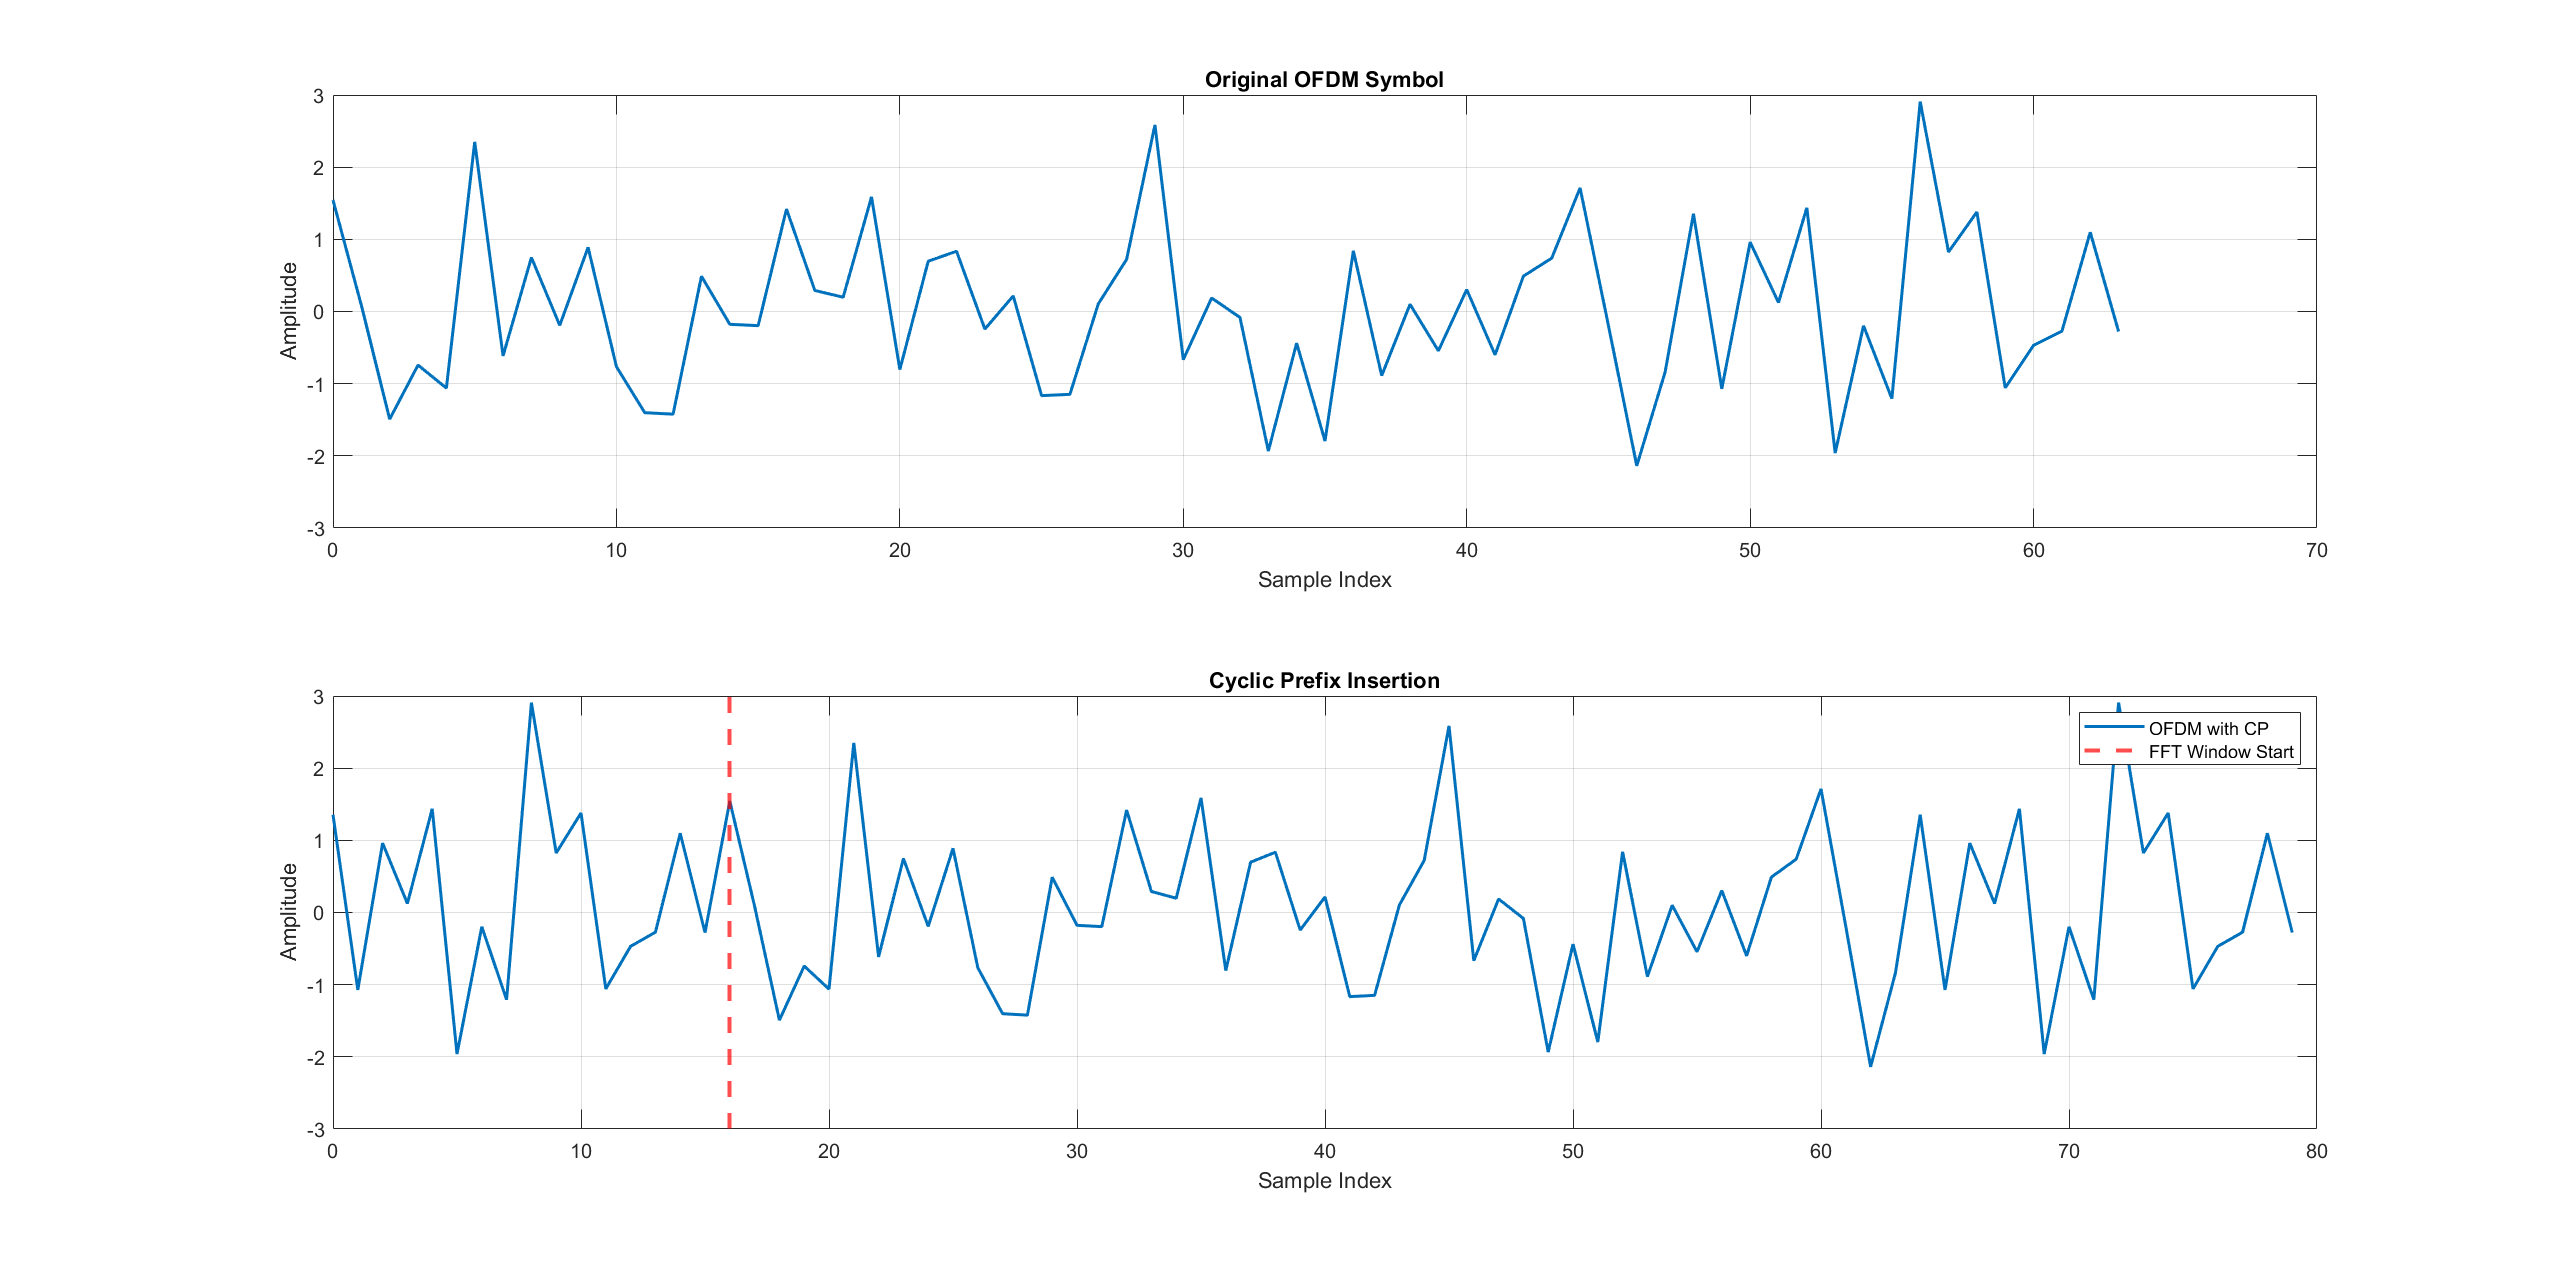
\includegraphics[width=1.3\textwidth]{Figures/cp_insertion.png}
    \caption{\bfseries Cyclic prefix insertion process}
    \label{fig:cp_insert}
\end{figure}

Figure \ref{fig:cp_insert} illustrates the cyclic prefix insertion process.
The samples before the red dashed line correspond to the cyclic prefix,
which is copied from the end portion of the OFDM symbol and appended to
the beginning before transmission. At the receiver, the cyclic prefix is
removed, and the FFT operation begins at the boundary marked by the red
line in order to recover the original OFDM symbol while mitigating
inter-symbol interference caused by multipath propagation.

%============================================================%
\subsection{Multipath Rayleigh Fading Channel}

A fixed three-tap Rayleigh fading channel was used throughout the
simulation.

The generated channel taps are:

\begin{equation}
h =
[-0.6341 - 0.1139i,\;
0.4427 + 0.5667i,\;
-0.2504 - 0.0712i]
\end{equation}

The total channel power was normalized:

\begin{equation}
\sum_{l=0}^{L-1}|h_l|^2 = 1
\end{equation}

The received signal is expressed as:

\begin{equation}
r[n]=x[n]*h[n]+w[n]
\end{equation}

where:
\begin{itemize}
    \item $x[n]$ is the transmitted signal,
    \item $h[n]$ is the channel impulse response,
    \item $w[n]$ is AWGN noise.
\end{itemize}

\vspace{0.3cm}

\begin{figure}[H]
    \centering
    \hspace*{-0.18\textwidth}
    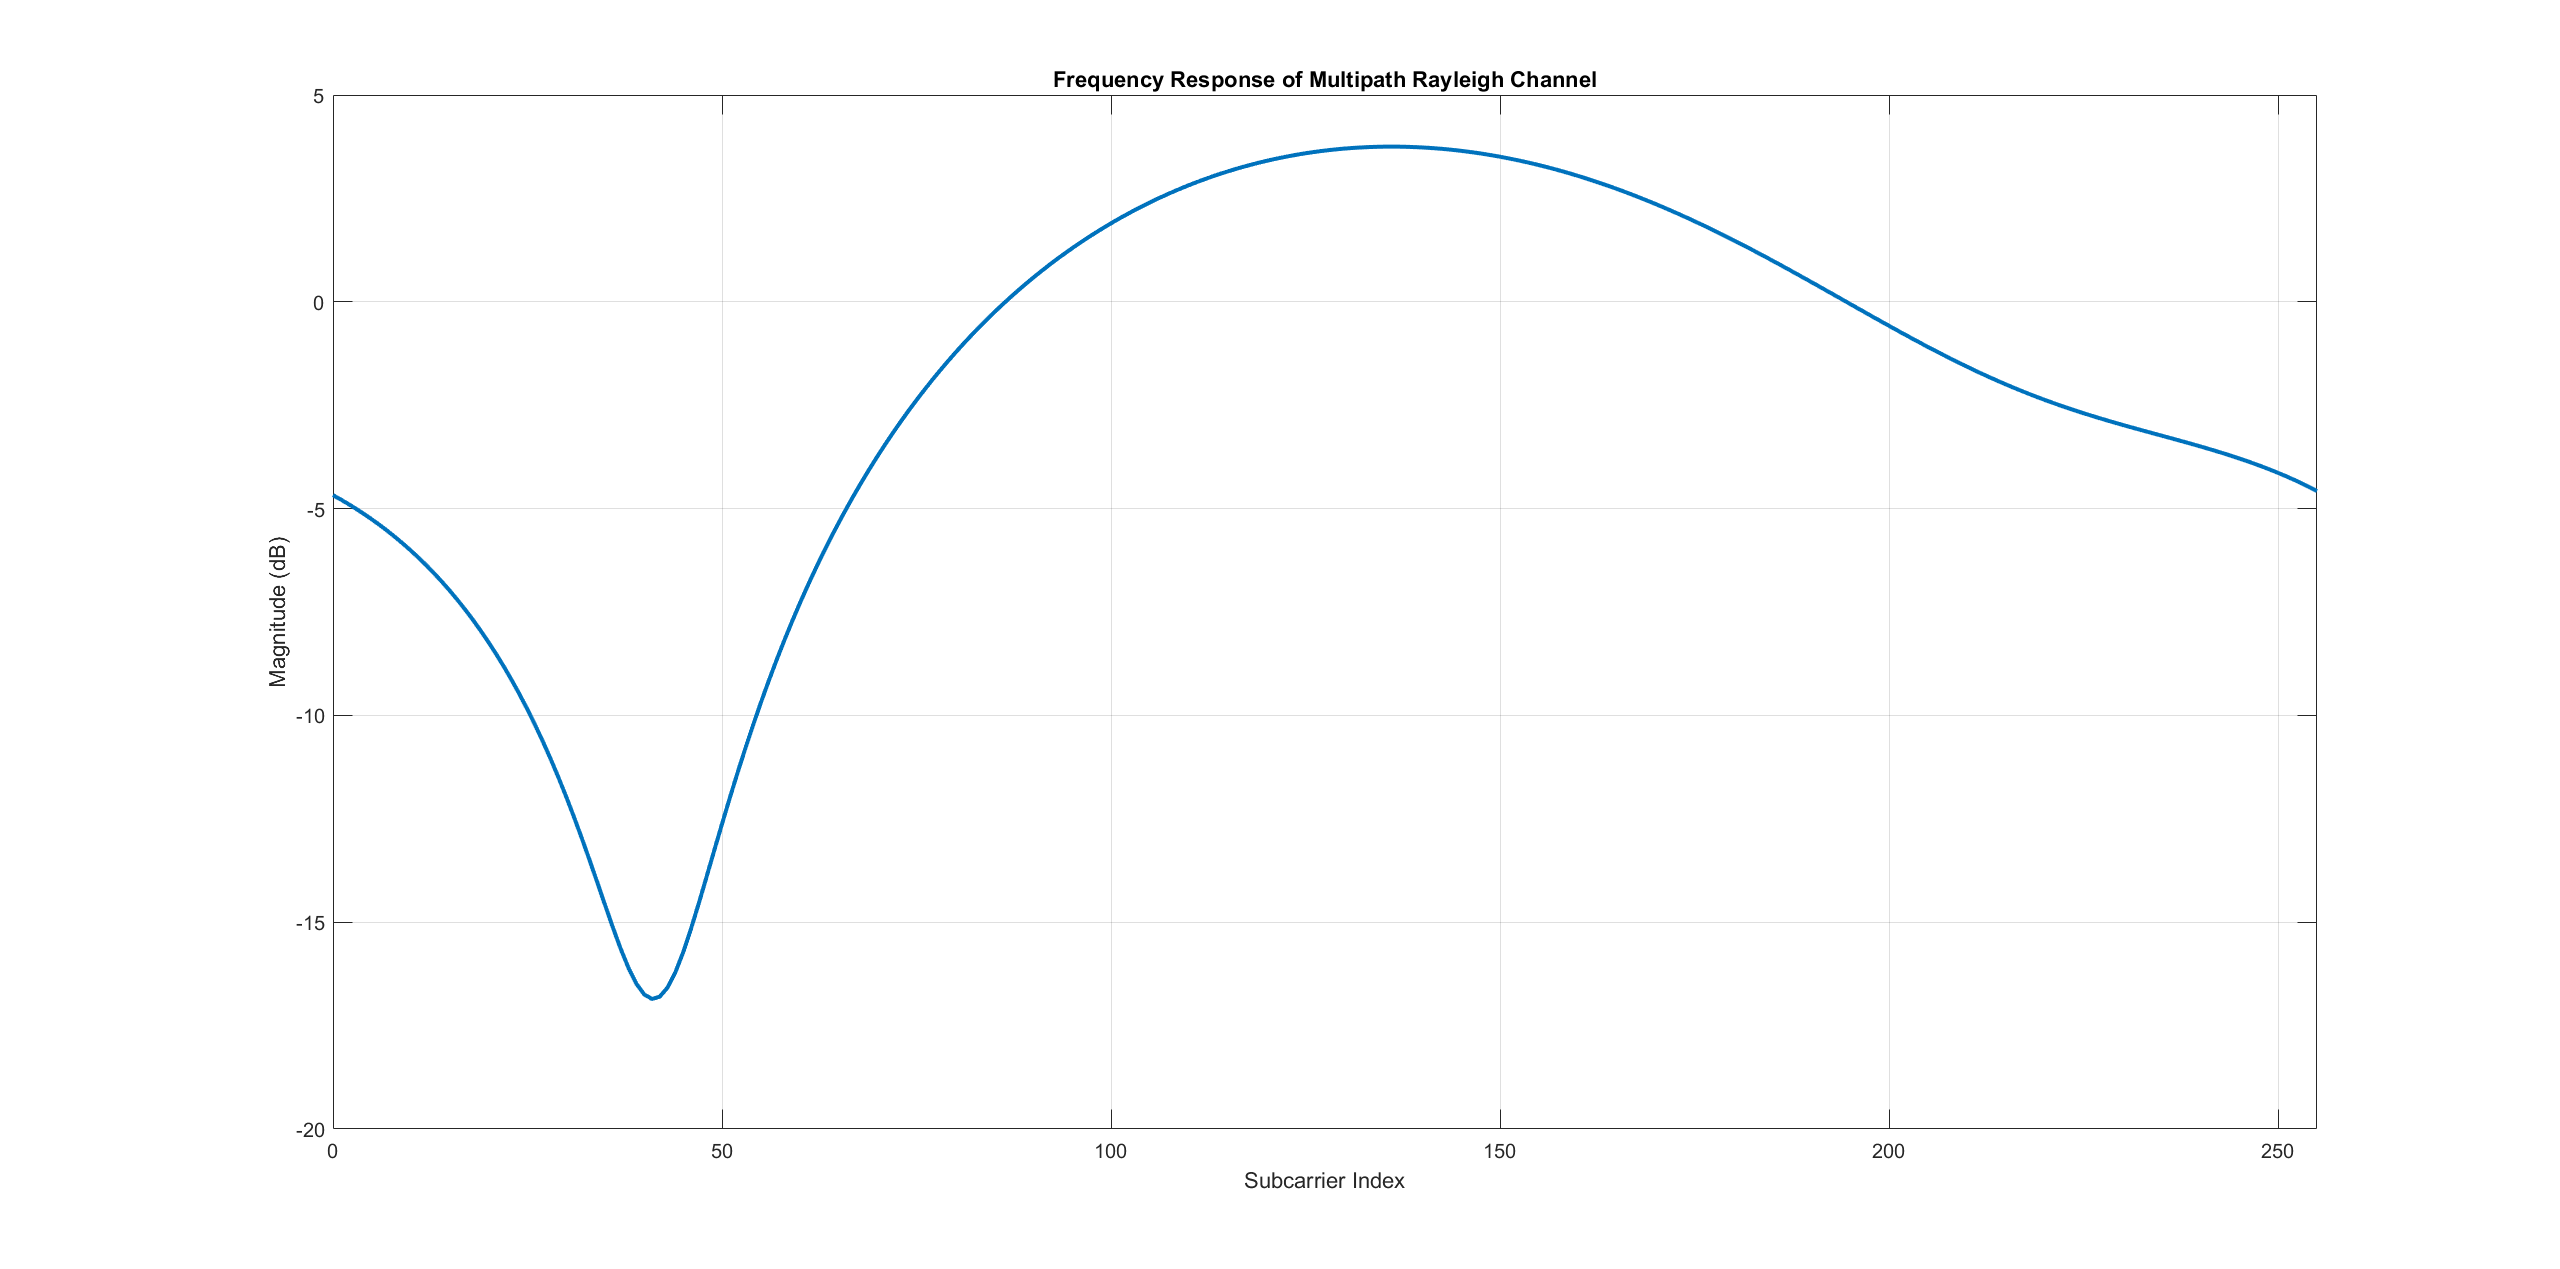
\includegraphics[width=1.3\textwidth]{Figures/channel_response.png}
    \caption{\bfseries Frequency response of the multipath channel}
    \label{fig:channel_response}
\end{figure}

Figure \ref{fig:channel_response} illustrates the frequency response of
the simulated three-tap Rayleigh fading channel used throughout the
experiment. Because the channel contains multiple delayed propagation
paths with different amplitudes and phases, the resulting frequency
response is non-uniform across the OFDM subcarriers.

It can be observed that several subcarriers experience lower channel gain
(deep fading regions), while others experience stronger constructive
combination of multipath components. These fluctuations demonstrate the
frequency-selective nature of the channel.

In practical communication systems, deep spectral fades may significantly
degrade detection performance on affected subcarriers. This characteristic
motivates the use of OFDM-based systems, where narrowband orthogonal
subcarriers and frequency-domain equalization simplify compensation for
multipath distortion.

The Signal-to-Noise Ratio (SNR) was varied from 0 dB to 20 dB to evaluate
system performance under different noise conditions.

%============================================================%
\subsection{Frequency-Domain Equalization}

After cyclic prefix removal and FFT processing, frequency-domain
equalization was applied.

The received subcarrier signal is:

\begin{equation}
Y[k]=H[k]X[k]+N[k]
\end{equation}

Zero Forcing equalization estimates the transmitted symbol using:

\begin{equation}
\hat{X}[k]=\frac{Y[k]}{H[k]}
\end{equation}

This operation compensates for channel distortion by dividing the received
signal by the channel frequency response.

For SC-FDMA, an additional IDFT despreading operation was applied after
equalization:

\begin{equation}
d[n]=\frac{1}{M}
\sum_{m=0}^{M-1}
X[m]e^{j\frac{2\pi mn}{M}}
\end{equation}

%============================================================%
\subsection{BER Evaluation Method}

Bit Error Rate (BER) was computed by comparing the transmitted bits with
the detected bits at the receiver.

\begin{equation}
\mathrm{BER}
=
\frac{N_e}{N_t}
\end{equation}

where:
\begin{itemize}
    \item $N_e$ is the number of erroneous bits,
    \item $N_t$ is the total number of transmitted bits.
\end{itemize}

The BER performance was evaluated for both OFDM and SC-FDMA systems over
the entire SNR range.

Table \ref{tab:ber_results} summarizes the obtained BER results.

\begin{table}[H]
\centering
\caption{BER Performance Comparison}
\label{tab:ber_results}
\begin{tabular}{|c|c|c|}
\hline
\textbf{SNR (dB)} & \textbf{OFDM BER} & \textbf{SC-FDMA BER} \\ \hline

0  & $1.859452\times10^{-1}$ & $2.249893\times10^{-1}$ \\ \hline
5  & $8.538000\times10^{-2}$ & $1.088427\times10^{-1}$ \\ \hline
10 & $2.599531\times10^{-2}$ & $2.228805\times10^{-2}$ \\ \hline
15 & $3.242734\times10^{-3}$ & $2.948438\times10^{-4}$ \\ \hline
20 & $2.992188\times10^{-5}$ & $0$ \\ \hline

\end{tabular}
\end{table}

\vspace{0.3cm}

\begin{figure}[H]
    \centering
    \hspace*{-0.18\textwidth}
    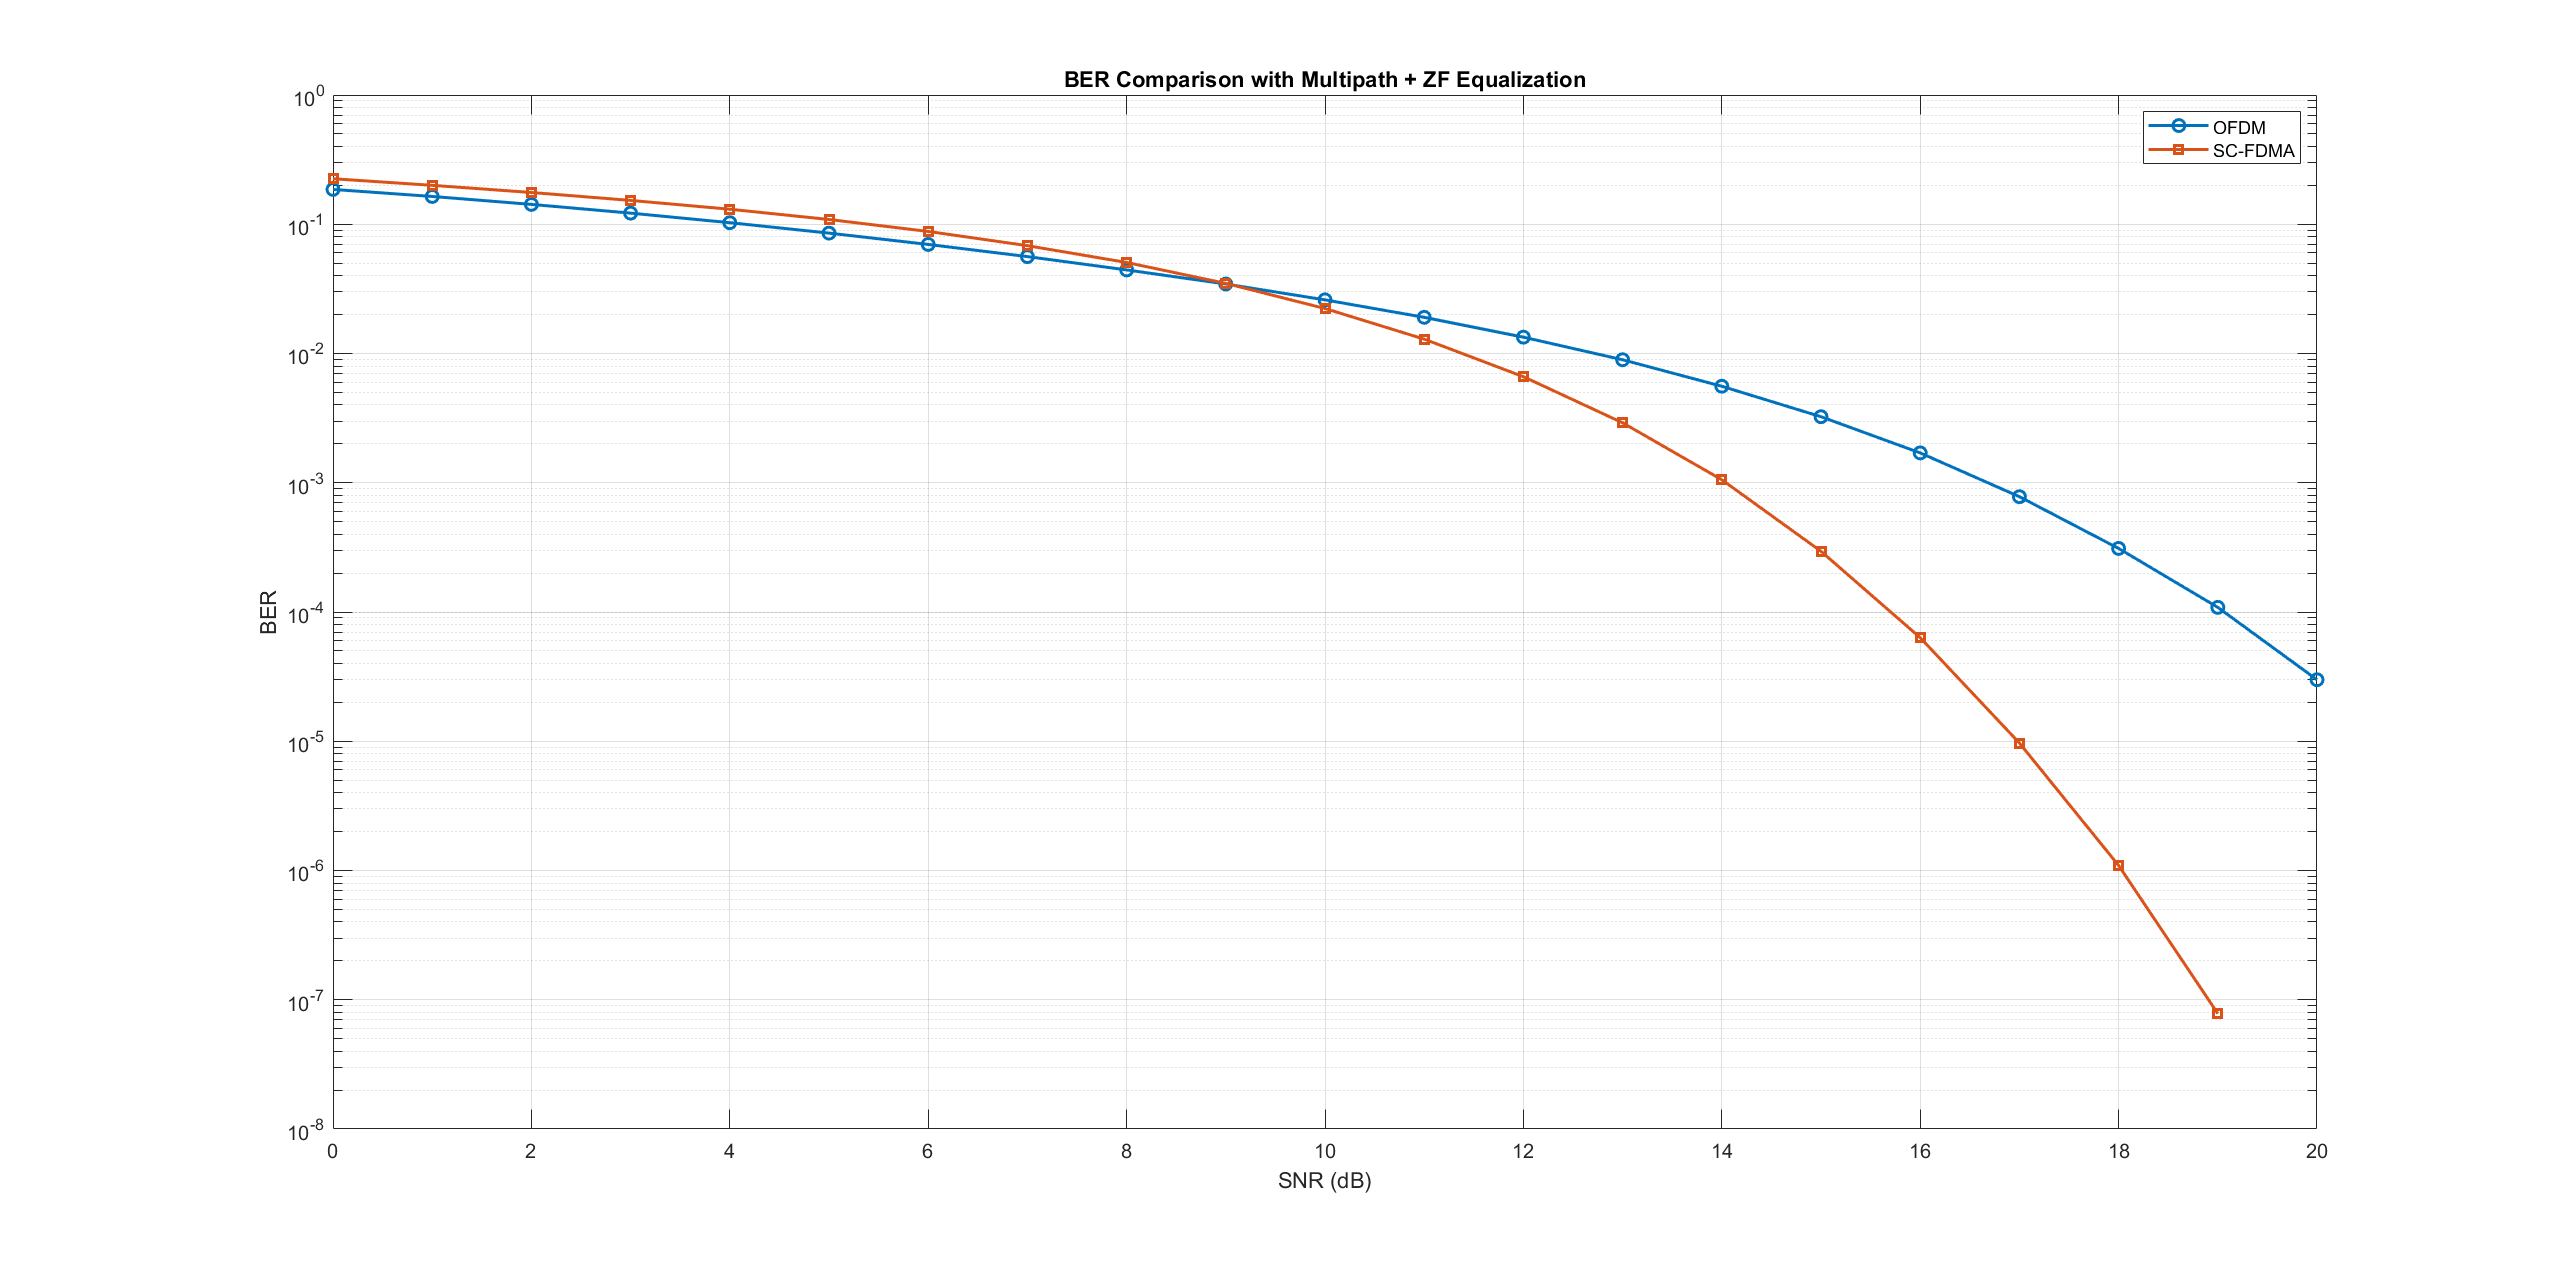
\includegraphics[width=1.3\textwidth]{Figures/ber_plot.png}
    \caption{\bfseries BER performance comparison between OFDM and SC-FDMA}
    \label{fig:ber_plot}
\end{figure}

%============================================================%
\subsection{PAPR and CCDF Evaluation}

PAPR measurements were performed for both OFDM and SC-FDMA transmitted
signals.

The PAPR is defined as:

\begin{equation}
\mathrm{PAPR}
=
\frac{\max |x[n]|^2}
{E\{|x[n]|^2\}}
\end{equation}

The Complementary Cumulative Distribution Function (CCDF) was used to
evaluate the probability that the PAPR exceeds a specified threshold:

\begin{equation}
\mathrm{CCDF}(P_0)
=
\Pr(\mathrm{PAPR}>P_0)
\end{equation}

The measured average PAPR values are:

\begin{table}[H]
\centering
\caption{Average PAPR Comparison}
\label{tab:papr_avg}
\begin{tabular}{|c|c|}
\hline
\textbf{System} & \textbf{Average PAPR (dB)} \\ \hline

OFDM & 6.0139 \\ \hline
SC-FDMA & 4.8222 \\ \hline

\end{tabular}
\end{table}

The results clearly show that SC-FDMA achieves significantly lower PAPR
than OFDM.

\vspace{0.3cm}

\begin{figure}[H]
    \centering
    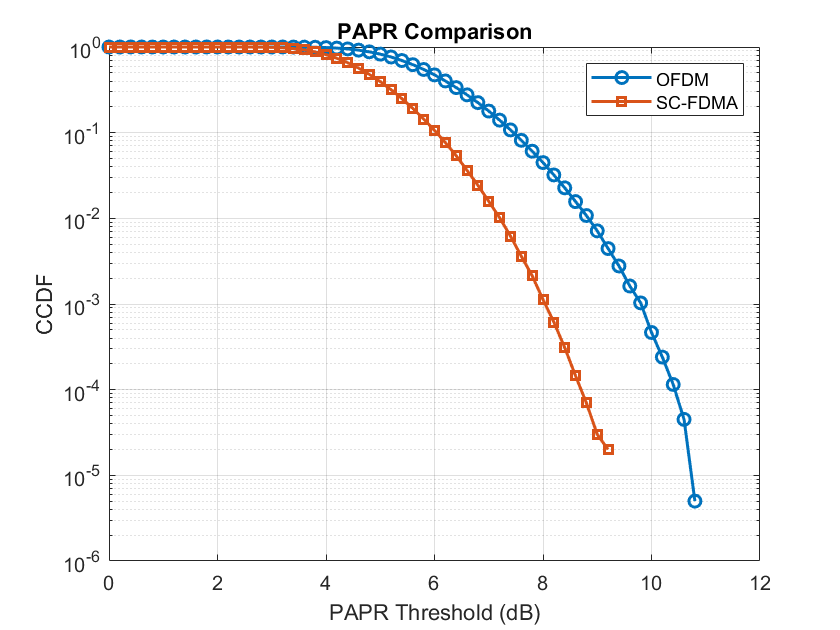
\includegraphics[width=0.92\textwidth]{Figures/papr_ccdf_plot.png}
    \caption{\bfseries CCDF comparison of OFDM and SC-FDMA PAPR}
    \label{fig:ccdf_plot}
\end{figure}

%============================================================%
\subsection{Computational Considerations}

A total of 200000 transmitted blocks were simulated for each SNR point.
The simulation therefore required a large computational workload to obtain
statistically reliable BER and CCDF results.

Progress indicators were implemented during execution to monitor the
simulation status:

\begin{center}
\texttt{SNR = 10 dB | Processing block 100000 / 200000}
\end{center}

The use of a fixed channel realization ensured fair comparison between
OFDM and SC-FDMA under identical fading conditions.

%============================================================%
\subsection{Chapter Summary}

This chapter presented the MATLAB simulation framework used to compare
OFDM and SC-FDMA systems under multipath Rayleigh fading channels.

The transmitter structure, cyclic prefix operation, channel model,
frequency-domain equalization, BER analysis, and PAPR evaluation methods
were described in detail.

The next chapter presents a detailed discussion and interpretation of the
simulation results.